\documentclass[12pt]{beamer}
\usepackage{CJK}
\usepackage{beamerthemeshadow} %该为一现成的模板,在 MiKTeX\texmf\tex\latex\beamer\themes\theme下面有很多
\usetheme{Warsaw} %{Madrid}

\title{Sliders' title 标题}
\author{Hu Qinghai作者}
\date{\today}

\begin{document} %申明文档的开始
\begin{CJK}{UTF8}{gbsn}     %CJK:支持中文
    \begin{frame} %beamer里重要的概念,每个frame定义一张page
        \titlepage   
    \end{frame}

    \begin{frame}
        \frametitle{目录}
        \begin{itemize}
         \item 背景介绍 \pause
         \item 热点分析 \pause
		 \item 优化方法 \pause
         \item 效果分析 \pause
		 \item 总结
        \end{itemize}
        \tableofcontents
    \end{frame}

    \begin{frame}
        \frametitle{背景介绍}
        \pause
        Qt画线程序是....
        \begin{definition}
            definition定义 1...
        \end{definition}
    \end{frame}

    \begin{frame}
        \frametitle{热点分析}\pause
        \begin{itemize}
         \item beamer introd tion \pause
         \item beamer details \pause
         \item beamer conclusions
        \end{itemize}
    \end{frame}

    \begin{frame}
        \frametitle{效果分析}\pause
		\begin{figure}[!htbp]
			\centering
			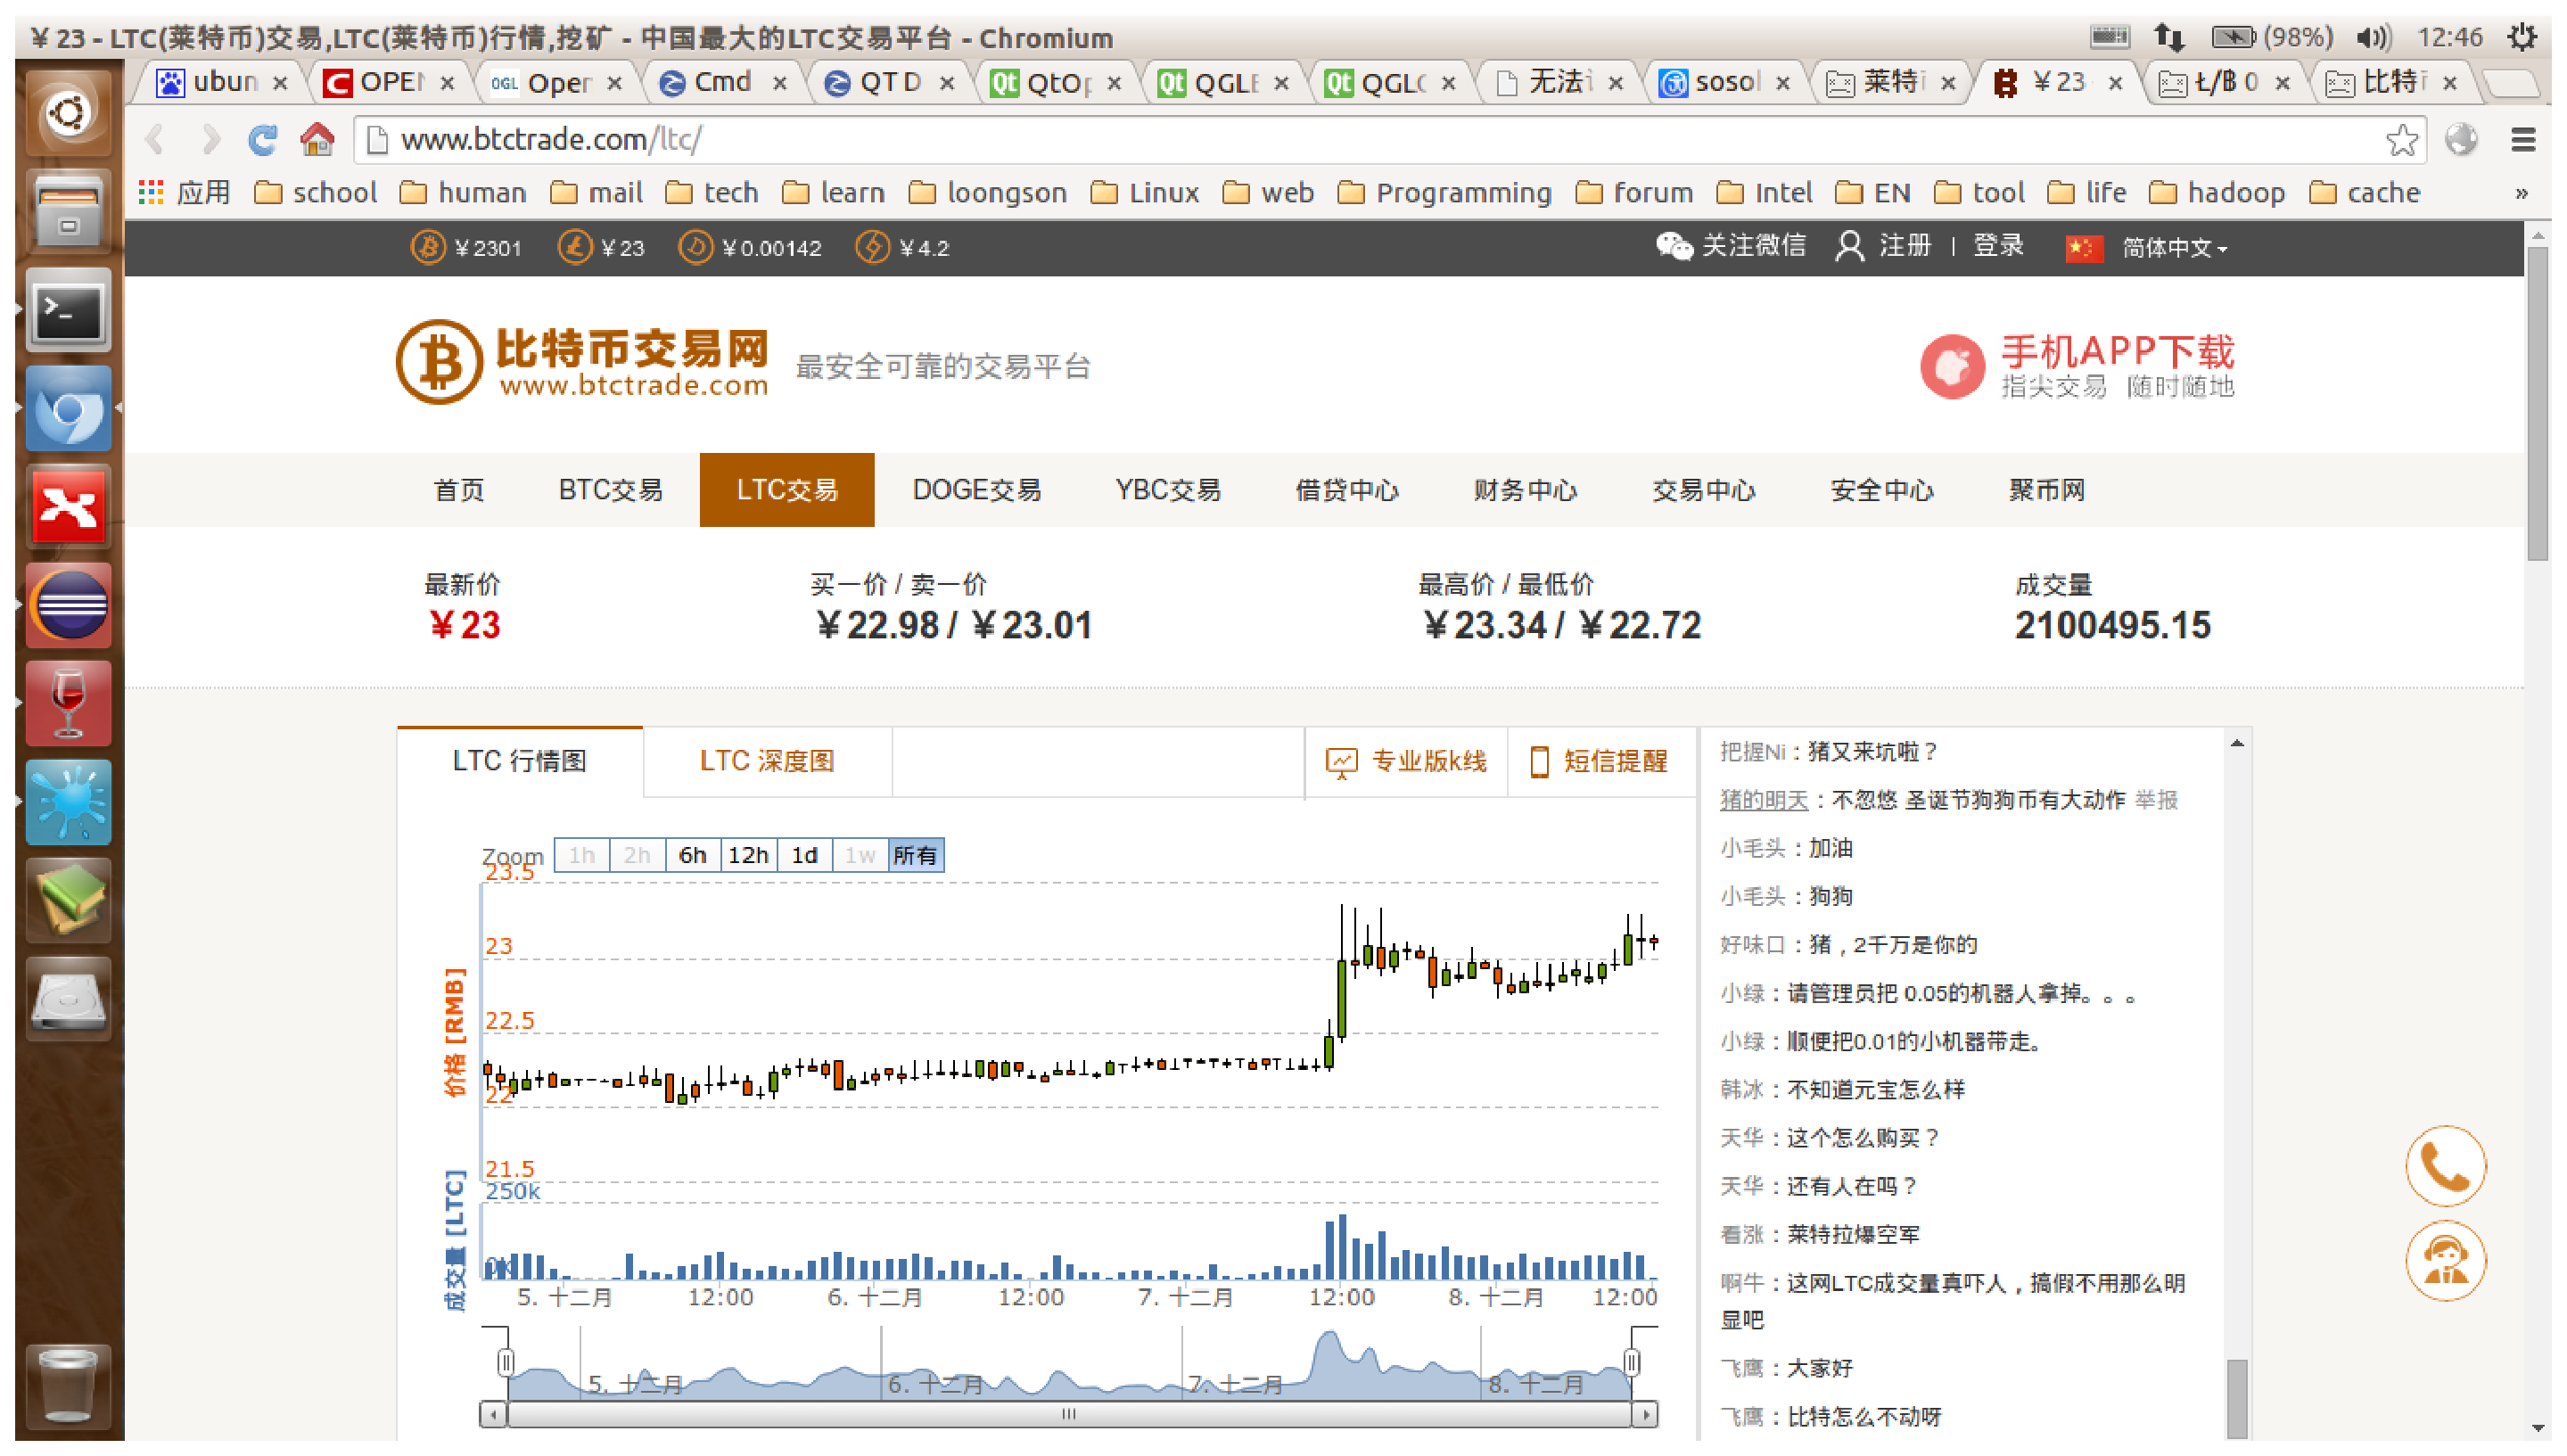
\includegraphics[width=10.00cm,height=7.10cm]{test.eps}
			\caption{一个图}
		\end{figure}
    \end{frame}

	\begin{frame}
		\frametitle{定理}
		\begin{lemma}[1]
		这是一个定理,引理类似。
		\end{lemma}
		\pause                       % 这里会暂停一下,pagedown会接着出现下面的式子
		\begin{displaymath}             %这个不用解释了吧
		1+1=2
		\end{displaymath}
		\begin{equation}
		1+1=2
		\end{equation}
	\end{frame}

	\begin{frame}\frametitle{插个表}
	一个表.
	 \begin{table}
	  \centering \addtolength{\tabcolsep}{1mm}
	 \begin{tabular}{ccccccccc}
	   \hline
	        & 1 & 2 & 3 & 4 & 5 & 6 & 7 & 8 \\
	   \hline
	    1 &         &       &          &       &       &       &       &  \\
	    2 & $c$     &       &          &       &       &       &       &  \\
	    3 & $c$     & $c $  &          &       &       &       &       &  \\
	    4 & $a$     & $a,c$ & $a $     &       &       &       &       &  \\
		5 & $a,b,c$ & $a,b$ & $a,b,c$  & $b,c$ &       &       &       &  \\
   		6 & $a,c$   & $a,c$ & $a,c$    & $c $  & $b,c$ &       &       &  \\
   		7 & $a,b,c$ & $a,b$ & $a,b,c$  & $b,c$ &       & $b,c$ &       &  \\
   		8 & $a,c$   & $a,c$ & $a,c$    & $c$   & $b,c$ &       & $b,c$ &  \\
   		\hline
		\end{tabular}\label{dismatrix}
		\end{table}
		\end{frame}

	\begin{frame}\frametitle{参考文献}
		[1] A\newline
		[2] B
	\end{frame}

	\begin{frame}\frametitle{致谢}
		Thanks
	\end{frame}

\end{CJK}
\end{document}
